% --- InternVideo ---
% % % --- Video Foundation Model: InternVideo ---
\begin{frame}{Video Foundation Model: InternVideo2}
  \begin{itemize}
    \item Large-scale pre-trained video foundation model (InternVideo family; InternVideo2, Wang et al., 2024).
    \item Developed to generalize across diverse video understanding tasks by learning rich spatio-temporal features adaptable to unseen video domains.
    \item Capabilities: Recognition, localization, captioning, segmentation, search, QA, and multi-modal video reasoning.
    \item Complements last lecture's V-JEPA 2: same goal of general video representations, but built from masked reconstruction plus contrastive alignment rather than latent prediction.
  \end{itemize}
\end{frame}

\begin{frame}{InternVideo2: How It Works}
  \begin{itemize}\footnotesize
        \item Stage 1: Spatiotemporal perception (masked reconstruction)
        \item Stage 2: Semantic alignment (video-text/audio contrastive learning)
        \item Stage 3: World-modeling style reasoning (next-token objectives)
  \end{itemize}
  \centering
  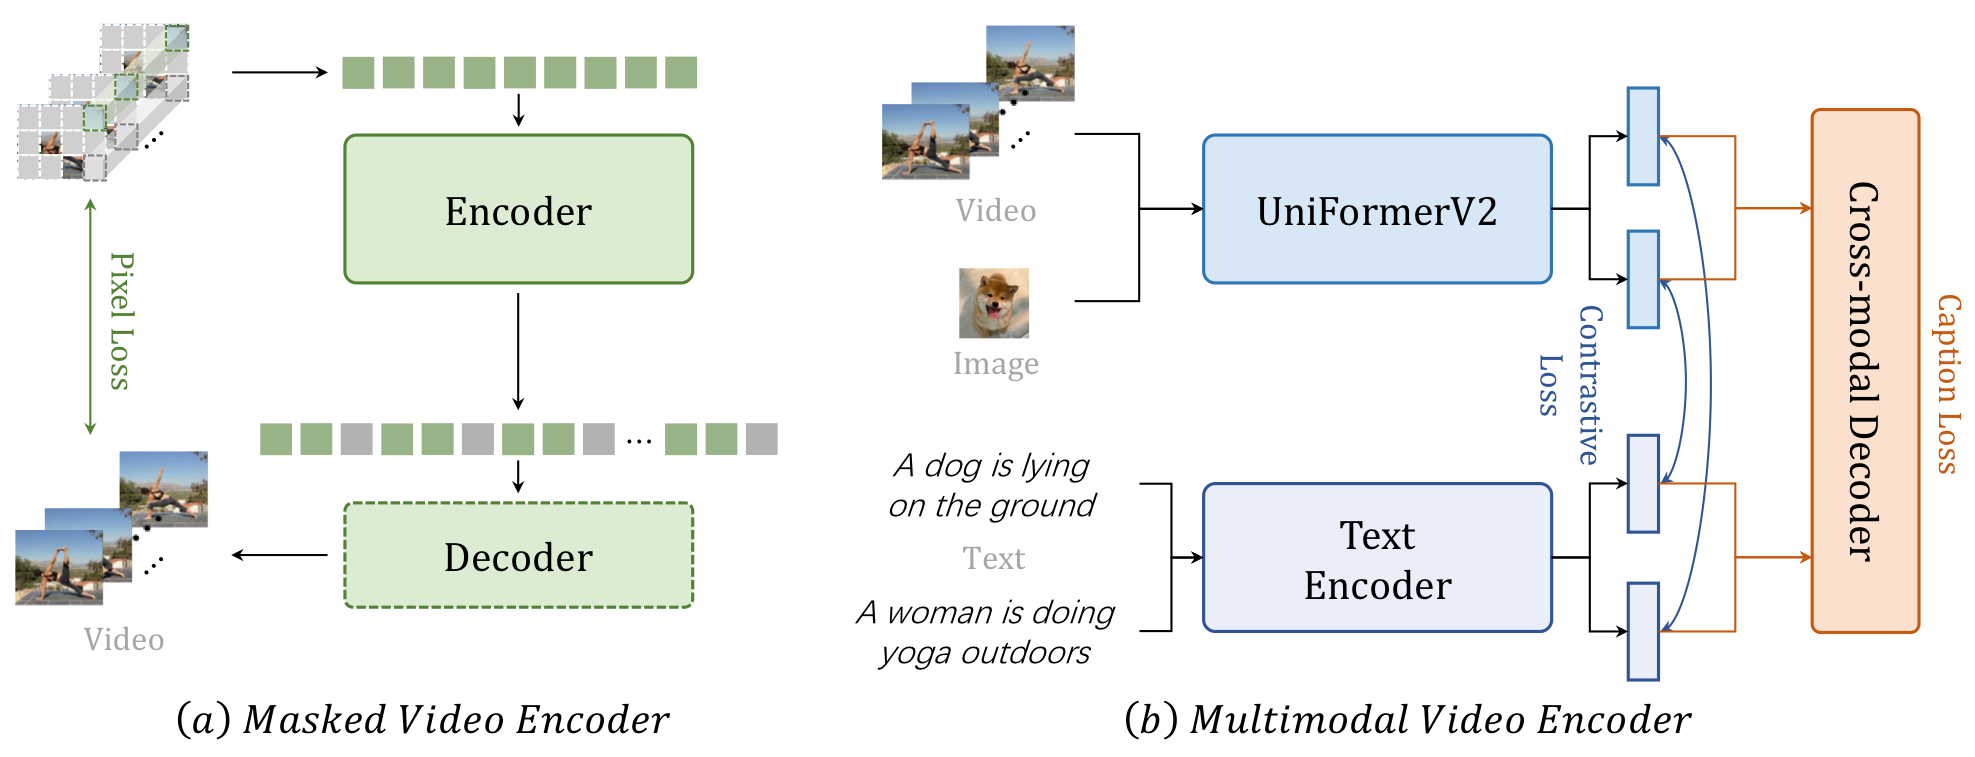
\includegraphics[width=0.8\textwidth]{images/foundation-models/internvideo.png}\\[0.25em]
  {\scriptsize Figure from the InternVideo2 paper: architecture overview.}
\end{frame}
